\chapter{Agentes inteligentes}
\label{cap:agentes-inteligentes}

\framebox[\textwidth]{
	\hspace{1em}
	\vbox{
		\textbf{Leitura obrigatória:}
		\begin{itemize}
			\item \cite{RusselAndNorvig2010} -- Cap. 2 (Introdução).
		\end{itemize}
		
		\textbf{Leitura complementar:}
		\begin{itemize}
			\item \cite{Wooldridge2009} -- Cap. 2 (Intelligent Agents).
		\end{itemize}
	}
}

\section{Por que agentes?}

Muitos pesquisadores da área da inteligência artificial utilizam o conceito de agentes na construção de um sistema inteligente. Uma entidade computacional é, portanto, um agente que percebe seu ambiente e atua sobre ele em busca do seu objetivo. Dessa forma, podemos pensar em \textbf{agentes inteligentes} e \textbf{agentes racionais}, fazendo uso das ideias apresentadas no Capítulo~\ref{cap:introducao}. \citet{RusselAndNorvig2010} utilizam o conceito de agentes para definir um conjunto de princípios de projeto para a construção de sistemas inteligentes e norteiam o estudo da inteligência artificial em função destes conceitos. Logo, quando projetamos uma entidade dotada de inteligência artificial, estamos definindo um agente inteligente (ou agente racional).

\textbf{OBS:} existe uma vertente da inteligência artificial que estuda com maior profundidade os agentes inteligentes e os sistemas multiagente (sistema composto por um conjunto de agentes que interagem entre si). Para mais detalhes sobre este ramo, veja \citet{Weiss1999} e \citet{Wooldridge2009}.

\section{Conceitos básicos}

Esta seção apresenta os conceitos fundamentais de agentes inteligentes e ambientes, bem como sua relação com a construção de sistemas inteligentes.

\subsection{O que é um agente?}

\citet{RusselAndNorvig2010} definem agente como uma entidade (de software ou não) capaz de perceber seu \textbf{ambiente} por meio de \textbf{sensores} e atuar sobre o ambiente por meio de \textbf{atuadores}. Considerando ambiente como um provedor de entradas e receptor de saídas, podemos concluir que qualquer programa é um agente (tudo é um agente). Este conceito será utilizado no decorrer deste material, para a definição de agentes capazes de realizar tarefas com o uso de conceitos de inteligência artificial. No entanto, alguns autores questionam esta definição genérica de agentes, incluindo algumas características que diferem um simples programa computacional de um agente. \citet{FranklinAndGraesser1996} apresentam definições de vários autores e discutem sobre os pontos em comum e as diferenças nos conceitos fundamentais da área.

\textbf{Definição de \citet{FranklinAndGraesser1996}}
\begin{quotation}
``\textit{an \textbf{autonomous} agent is a system situated within and a part of an \textbf{environment} that \textbf{senses} that environment and \textbf{acts} on it, over time, in pursuit of its own \textbf{agenda} and so as to affect what it senses in the future}.''
\end{quotation}

\insertspace

\textbf{Definição de \citet{Wooldridge2009}}
\begin{quotation}
``\textit{a computer system that is situated in some \textbf{environment} and that is capable of independent (\textbf{autonomous}) \textbf{action} in this environment on behalf of its user or owner (figuring out what needs to be done to satisfy design \textbf{objectives}, rather than constantly being told)}.''
\end{quotation}

\insertspace

Algumas características gerais podem ser listadas a partir dessas definições:

\begin{itemize}
	\item O agente sempre está situado em um ambiente, percebe (sensores) seu estado e atua (atuadores) sobre ele.
	\item O agente deve ser autônomo, isto é, toma suas próprias decisões.
	\item O agente possui um objetivo, que conduz a sua tomada de decisões.
\end{itemize}

\insertspace

\begin{figure}[h]
	\centering
	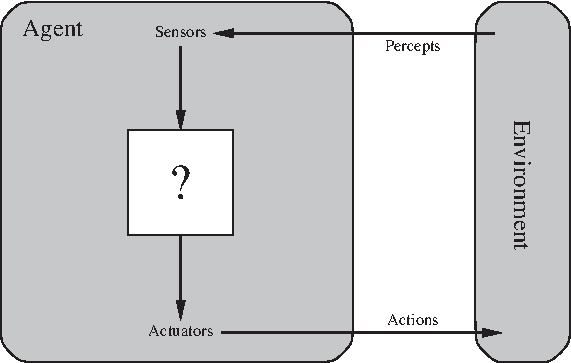
\includegraphics[width=0.5\textwidth]{img/agente-ambiente}
	\caption{Esquema geral de um agente e seu ambiente}
	\label{fig:agente-ambiente}
\end{figure}

A Figura~\ref{fig:agente-ambiente} apresenta o esquema geral de um agente e sua interação com o ambiente no qual está situado. O agente percebe o estado do seu ambiente através de sensores, infere sobre o que deve ser feito (tomada de decisão), e atua sobre o ambiente por meio de seus atuadores. A caixa representada por um sinal ``\textbf{?}'' define o funcionamento interno do agente. Ou seja, este elemento representa a implementação do agente, sua autonomia, seus objetivos e as técnicas de inteligência artificial utilizada por ele.

\subsection{Comportamento dos agentes}

Uma vez conhecido o conceito de agente, uma parte importante do seu projeto e implementação é a determinação do seu comportamento. Ou seja, como o agente processa as entradas, toma decisões e atua sobre o ambiente. A \textbf{percepção} é, portanto, aquilo que o agente enxerga do seu ambiente (seu estado). Um agente pode escolher uma ação não somente em função da sua percepção atual, mas da sequência de percepções obtidas anteriormente. A esta sequência de percepções damos o nome de história do agente.

Uma das formas de definirmos o comportamento do agente é através da construção de uma tabela que mapeia sequências de percepções para as ações desejadas. Este mapeamento é chamado de \textbf{função do agente} e sua implementação é chamada \textbf{programa do agente}. Na maioria dos casos, esta tabela seria infinita e, portanto, uma tabulação completa é impossível.

\textbf{Exemplo -- agente aspirador de pó:} o agente consiste em um robô cuja tarefa é aspirar o pó do chão. O ambiente é composto por dois quadrados (A e B). O agente percebe em qual quadrado está e se há sujeira, e pode (1) mover-se para a direita, (2) mover-se para a esquerda, (3) aspirar a sujeira ou (4) não fazer nada. A Figura~\ref{fig:agente-aspirador} ilustra o cenário apresentado.

\begin{figure}[h]
	\centering
	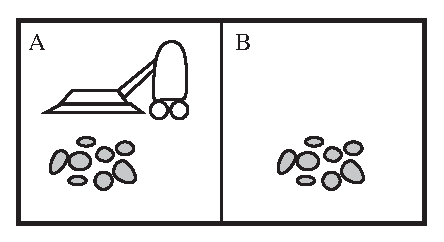
\includegraphics[width=0.5\textwidth]{img/agente-aspirador.eps}
	\caption{Agente aspirador e seu ambiente}
	\label{fig:agente-aspirador}
\end{figure}

A Tabela~\ref{tab:tabulacao-agente-aspirador} apresenta a função de agente do robô aspirador. Neste caso, a história completa do agente não é relevante. Basta ele perceber o estado do quadro em que se encontra (sujo ou limpo), para decidir sobre qual ação executar. No entanto, outras situações podem fazer uso do histórico para inferir sobre qual a melhor ação possível. Um ponto importante é: \textit{qual a melhor função de agente possível?} Ou seja, o que torna o agente bom ou ruim, inteligente ou não?

\begin{table}[h]
	\centering
	\begin{tabular}{p{13cm}l}
		\hline
		\textbf{Sequência de percepções} & \textbf{Ação} \\
		\hline
		$[$\textit{A}, \textit{Limpo}$]$ & \textit{Direita} \\
		$[$\textit{A}, \textit{Sujo}$]$ & \textit{Aspirar} \\
		$[$\textit{B}, \textit{Limpo}$]$ & \textit{Esquerda} \\
		$[$\textit{B}, \textit{Sujo}$]$ & \textit{Aspirar} \\
		$[$\textit{A}, \textit{Limpo}$]$, $[$\textit{A}, \textit{Limpo}$]$ & \textit{Direita} \\
		$[$\textit{A}, \textit{Limpo}$]$, $[$\textit{A}, \textit{Sujo}$]$ & \textit{Aspirar} \\
		$\vdots$ & $\vdots$ \\
		$[$\textit{A}, \textit{Limpo}$]$, $[$\textit{A}, \textit{Limpo}$]$, $[$\textit{A}, \textit{Limpo}$]$ & \textit{Direita} \\
		$[$\textit{A}, \textit{Limpo}$]$, $[$\textit{A}, \textit{Limpo}$]$, $[$\textit{A}, \textit{Sujo}$]$ & \textit{Aspirar} \\
		$\vdots$ & $\vdots$ \\
		\hline
	\end{tabular}
	\caption{Função de agente do robô aspirador}
	\label{tab:tabulacao-agente-aspirador}
\end{table}

Para definir o quão bom um agente é na realização de uma tarefa, precisamos de uma \textbf{medida de desempenho}, que determina o sucesso do comportamento de um agente, geralmente expresso quantitativamente. Em muitos casos chamaremos esta medida de \textbf{função objetivo}. Esta medida de desempenho deve ser imposta pelo projetista e, em geral, diz respeito ao estado do ambiente após a sequência de ações executadas pelo agente. Se o estado do ambiente é o estado desejado para a tarefa, o agente obteve sucesso. Nem sempre a definição da medida de sucesso é uma tarefa simples.

No exemplo do agente aspirador de pó, as seguintes medidas de sucesso poderiam ser definidas:
\begin{itemize}
	\item \textbf{\textit{Quantidade de sujeira limpa por dia}:} o agente pode repetir as ações de limpar a sujeira e jogá-la novamente no chão, maximizando sua medida de desempenho.
	\item \textbf{\textit{Quantidade de quadrados limpos no final do dia}:} o agente se limitaria a manter os dois quadrados limpos.
	\item \textbf{Conclusão:} é importante planejar a medida de desempenho em função da real expectativa de resultado.
	\item \textbf{Questões adicionais:} e se, além do chão limpo, quiséssemos minimizar o consumo de energia elétrica e a emissão de ruído?
\end{itemize}

\insertspace

Com base nestas informações, o conceito de \textbf{racionalidade} consiste em tomar a melhor decisão possível, levando em consideração os seguintes aspectos:
\begin{itemize}
	\item A medida de desempenho (critério de sucesso)
	\item O conhecimento do agente sobre o ambiente
	\item As ações que o agente pode executar
	\item A sequência de percepções do agente até o momento
\end{itemize}

\insertspace

Um \textbf{agente racional} é, portanto, um agente que toma suas decisões com racionalidade. Ou seja, um agente racional toma a melhor decisão que pode, conforme sua medida de desempenho, seu conhecimento, suas ações e percepções. \citet{RusselAndNorvig2010} apresentam uma definição formal para um agente racional:

\begin{quotation}
	\textit{``Para cada sequência de percepções possível, um agente racional deve selecionar uma ação que se espera venha a maximizar sua medida de desempenho, dada a evidência fornecida pela sequência de percepções e por qualquer conhecimento interno do agente.''}
\end{quotation}

Considere um agente aspirador de pó que limpa um quadrado se ele estiver sujo e passa para o outro quadrado se o primeiro não estiver sujo (repetidamente executa esta sequência de ações). Para definir se o mesmo é ou não racional, é necessário analisar o contexto no qual o agente se encontra segundo os fatores envolvidos no conceito de racionalidade (apresentados acima).
\begin{itemize}
	\item \textbf{Medida de desempenho:} o agente recebe um ponto para cada quadrado limpo ao fim do dia, ao longo de uma duração de 1000 dias;
	\item \textbf{Conhecimento do agente sobre o ambiente:} o agente conhece a ``geografia'' do ambiente e desconhece sua posição inicial e a distribuição da sujeira. Quadrados limpos permanecem limpos até o fim do dia. A ação de aspiração limpa o quadrado atual. As ações \textit{esquerda} e \textit{direita} movem o agente para o quadrado ao lado (conforme lado escolhido). O agente não pode movimentar-se para fora do ambiente.
	\item \textbf{As ações disponíveis:} \textit{esquerda}, \textit{direita}, \textit{aspirar} e \textit{nada} (não fazer nada).
	\item \textbf{Sequência de percepções:} o agente percebe sua posição e se a posição contém sujeira.
\end{itemize}

Podemos concluir que o agente em questão é racional, pois obterá a máxima pontuação possível (medida de desempenho) executando o comportamento apresentado. No entanto, se adicionarmos novas circunstâncias ao cenário, este mesmo agente pode passar a ser irracional. Se a medida de desempenho incluir o consumo de energia, existem funções de agente melhores (que não oscilam entre os quadrados após estarem limpos).

\subsection{Conceitos adicionais}

É importante destacar a diferença entre um agente racional e um agente onisciente (\textbf{racionalidade não é onisciência}). Um agente racional escolhe ações que maximizam a sua recompensa (maximiza a sua medida de desempenho). No entanto, em ambientes reais (ou suficientemente complexos) existem fatores externos ao conhecimento e percepções do agente, que podem afetar o resultado de uma ação. Por exemplo, o agente aspirador de pó pode selecionar a ação aspirar sem saber que junto da sujeira encontra-se uma substância danosa ao seu funcionamento. Neste caso, uma vez que o chão contém sujeira e o agente não sabe da substância danosa, a ação racional é aspirar a sujeira. Esta ação, mesmo que racional, leva a um resultado muito ruim.

Por outro lado, um agente onisciente possui conhecimento completo do contexto no qual está inserido. Ele decide sobre suas ações considerando todas as variáveis que podem influenciar no resultado final (em um valor menor ou maior de medida de desempenho). Em resumo, um agente racional maximiza o \textit{retorno esperado} de suas ações, enquanto um agente onisciente maximiza o \textit{retorno real} de suas ações.

Como na maior parte das vezes um agente racional não conhece completamente seu ambiente, uma estratégia racional é tomar ações que o permitam coletar informações. Por exemplo, o agente aspirador de pó poderia, antes de selecionar a ação \textit{aspirar}, executar a ação \textit{verificar}, que checa se existe alguma substância danosa na sujeira. Ou ainda, se modificarmos o ambiente deste agente para um conjunto de quadrados desconhecidos, o agente deveria executar ações de \textbf{exploração} do ambiente.

Paralelo às habilidades de coleta de informações e de exploração, um agente deve ser capaz de \textbf{aprender} ao longo do tempo. Em geral, o agente já possui um conhecimento prévio do ambiente, definido pelo projetista. Se este conhecimento for parcial e/ou limitado, ou ainda se o ambiente muda com o passar do tempo, um agente sem capacidade de adquirir novos conhecimentos dificilmente resolverá a tarefa com qualidade. Aprender significa utilizar a experiência para atualizar seu comportamento.

Quando um agente se comporta com base estritamente no conhecimento definido pelo projetista, este agente não possui \textbf{autonomia}. A medida que o agente aprende e passa a se comportar com base no conhecimento adquirido, dizemos que o agente é autônomo. Neste sentido, o agente inicialmente possui pouco conhecimento e a habilidade de aprender. Com o passar do tempo, o agente, autônomo e racional, pode se tornar independente do seu conhecimento prévio.

\section{O ambiente dos agentes}

Esta seção define o ambiente dos agentes e apresenta algumas propriedades destes ambientes, que o tornam mais ou menos complexos e impactam no projeto e implementação de agentes.

\subsection{Ambiente de tarefa}

O primeiro passo no projeto de um agente inteligente é a definição do seu \textbf{ambiente de tarefa}, composto pela medida de desempenho, ambiente, atuadores (ações) e sensores (percepções) do agente. Apesar do simples exemplo do aspirador de pó, a maioria dos ambientes são complexos e possuem características que dificultam a tarefa a ser executada (o que torna desafiador o campo de estudo da inteligência artificial). A Tabela~\ref{tab:ambientes-tarefa} apresenta alguns exemplos de ambientes de tarefa com diferentes níveis de complexidade.

\begin{table}[h]
	\centering
	\small
	\rowcolors{2}{white}{gray!25}
	\begin{tabular}{L{2cm} L{3cm} L{3cm} L{2.9cm} L{2.9cm}}
		\hline
		\rowcolor{black}
		\color{white}\textbf{Agente} & \color{white}\textbf{Medida de desempenho} & \color{white}\textbf{Ambiente} & \color{white}\textbf{Atuadores} & \color{white}\textbf{Sensores} \\
		\hline
		Veículo autônomo & Viagem segura, rápida, dentro da lei, minimizando tempo e consumo & Estradas, tráfego, pedestres, sinalização & Pedais, direção, sinal, buzina & Câmeras, sonar, velocímetro, GPS, hodômetro e acelerômetro  \\
		Sistema de diagnóstico médico & Acerto da doença, minimizar custos & Paciente, hospital, equipe & Painel de exibição de perguntas, testes, diagnósticos, tratamentos e indicações & Teclado para informar os sintomas \\
		Sistema de análise de imagens de satélite & Classificação correta da imagem & Link de transmissão & Monitor para exibir a categorização da imagem & Leitor de array de pixels \\
		Robô de seleção de peças & Percentual de peças na bandeja correta & Correia transportadora com peças, bandejas & Braço e mão articulados & Câmera, sensores angulares articulados \\
		Instrutor de inglês interativo & Maximizar nota do aluno em teste & Alunos, testes de agência & Monitor para exibir exercícios, sugestões e correções & Teclado para entrada de informações \\
		\hline
	\end{tabular}
	
	\caption{Exemplos de ambientes de tarefa}
	\label{tab:ambientes-tarefa}
\end{table}

Observações:
\begin{itemize}
	\item Alguns agentes são projetados para trabalhar em ambientes físicos (ex: veículo autônomo), enquanto outros se limitam a ambientes virtuais (ex: sistema de análise de imagens). Os agentes que operam exclusivamente em ambientes virtuais são chamados de \textbf{agentes de software}.
	
	\item Existem ambientes de tarefa (consequentemente os próprios agentes) simples e complexos, tanto em ambiente físico quanto virtual.
	\begin{itemize}
		\item \textbf{Agentes físicos:} aspirador de pó (simples) e robô para cuidado de pessoas idosas (complexo).
		\item \textbf{Agentes de software:} sistema para análise de palavras ofensivas em postagens (simples) e softbot para monitoramento do mercado financeiro (complexo).
	\end{itemize}
	
	\item A robótica é um importante (e vasto) campo de estudos no projeto e desenvolvimento de agentes físicos.
	
	\item Esta disciplina foca no estudo de agentes de software.
\end{itemize}

\subsection{Propriedades dos ambientes}

Os ambientes de tarefa podem ser classificados segundo seis dimensões. Estas dimensões balizam o projeto de agentes e a escolha da técnica de IA adequada para ele. Esta seção mostra a definição destas dimensões, as classificações existentes e alguns exemplos. Podemos adiantar que o caso mais difícil é um ambiente parcialmente observável, estocástico, sequencial, dinâmico, contínuo e multiagente (tenha isso em mente ao estudar as diferentes propriedades de cada dimensão). A tarefa de veículo autônomo, por exemplo, possui este nível de dificuldade.

\subsubsection{1. Completamente observável $\times$ parcialmente observável}

\begin{itemize}
	\item Se o agente consegue acessar o estado completo (ou pelo menos todas as informações que lhe importa) do ambiente, ele é completamente observável e, caso contrário, ele é parcialmente observável.
	
	\item Um ambiente pode ainda ser parcialmente observável quando as entradas são sensíveis a ruídos ou quando os sensores são imprecisos.
	
	\item \textbf{Aspirador de pó completamente observável:} o agente consegue observar todo o ambiente (dois quadrados).
	\item \textbf{Aspirador de pó parcialmente observável:} o agente possui um único sensor que só consegue verificar o quadrado atual.
\end{itemize}

\subsubsection{2. Determinístico $\times$ estocástico}

\begin{itemize}
	\item Se o próximo estado do ambiente é determinado pelo estado atual, mais a ação do agente, então o ambiente é determinístico. Se existem fatores externos que podem influenciar no próximo estado do ambiente, então ele é estocástico.
	
	\item Se o ambiente é determinístico exceto pelas ações de outros agentes, então ele é \textbf{estratégico}.
	
	\item \textbf{Aspirador de pó determinístico:} ele aspira a sujeira e o quadrado é limpo, os demais elementos do cenário permanecem no mesmo estado
	\item \textbf{Aspirador de pó estocástico:} o mecanismo de sucção não é confiável ou sujeira aparece aleatoriamente onde já estava limpo.
\end{itemize}

\subsubsection{3. Episódico $\times$ sequencial}

\begin{itemize}
	\item No caso episódico, a experiência do agente é dividida em episódios atômicos (iterações), onde o agente percebe o ambiente e executa uma ação. A escolha da ação do episódio não depende de episódios anteriores. No caso sequencial, uma ação pode modificar a escolha de ações futuras.
	
	\item Ambientes episódicos são mais simples, pois o agente não precisa pensar à frente. A classificação de uma peça não afeta a classificação das demais peças. Porém, uma jogada de xadrez pode afetar as demais jogadas e, por isso, o agente deve pensar nas consequências da ação no futuro.
	
	\item \textbf{Aspirador de pó episódico:} se o aspirador tivesse apenas a função de classificar um quadrado como sujo ou limpo.
	\item \textbf{Aspirador de pó sequencial:} considerando que a sujeira não retorna, a ação de limpar um quadrado implica no robô não precisar voltar ao referido quadrado no futuro.
\end{itemize}

\subsubsection{4. Estático $\times$ dinâmico}

\begin{itemize}
	\item O ambiente é dito estático quando ele não se altera com o passar do tempo. Isto é, desde que o agente percebe o ambiente até o momento da deliberação de uma ação, o ambiente possui o mesmo estado. Por outro lado, se o ambiente muda de estado enquanto o agente delibera, ele é dito dinâmico.
	
	\item Em ambientes dinâmicos o agente deve continuar observando o ambiente até decidir sobre uma ação, o que o torna mais complexo.
	
	\item Se o ambiente não muda ao longo do tempo, mas sim o nível de desempenho do agente, o ambiente é dito \textbf{semidinâmico}. Por exemplo, um jogo de xadrez com tempo se encaixa nesta classificação.
	
	\item \textbf{Aspirador de pó estático:} uma vez verificado o estado (limpo ou sujo), o ambiente não se altera.
	\item \textbf{Aspirador de pó dinâmico:} o agente pode perceber um quadrado limpo e, antes de tomar uma decisão, uma nova sujeira aparece no ambiente.
\end{itemize}

\subsubsection{5. Discreto $\times$ contínuo}

\begin{itemize}
	\item Este conceito se aplica a: (1) estado do ambiente, (2) modo como o tempo é tratado, ou ainda (3) percepções do agente. Ou seja, se o ambiente possui um número finito de estados discretos ou se ele é medido de forma contínua; se o tempo é discreto ou contínuo; se o agente percebe seu ambiente de forma discreta ou contínua.
	
	\item \textbf{Aspirador de pó discreto:} os estados são discretos (quadrado sujo ou quadrado limpo).
	\item \textbf{Aspirador de pó contínuo:} o agente poderia perceber a quantidade de sujeira, que poderia ser medida de forma contínua.
\end{itemize}

\subsubsection{Agente único $\times$ multiagente}

\begin{itemize}
	\item Quando o ambiente de tarefa envolve apenas um agente, o ambiente é dito de agente único, ou ainda \textbf{monoagente}. Quando diferentes agentes estão envolvidos no ambiente, temos um cenário multiagente.
	
	\item Um ambiente multiagente pode ser ainda \textbf{colaborativo}, quando o sucesso de um agente leva ao sucesso do outro agente, ou \textbf{competitivo}, quando o sucesso de um agente leva ao insucesso do outro agente.
	
	\item \textbf{Aspirador de pó de agente único:} um único aspirador de pó responsável pela limpeza do ambiente.
	\item \textbf{Aspirador de pó multiagente colaborativo:} dois ou mais aspiradores de pó responsáveis pela limpeza do ambiente, onde a medida de desempenho do agente é a área total limpa.
	\item \textbf{Aspirador de pó multiagente competitivo:} dois ou mais aspiradores de pó responsáveis pela limpeza do ambiente, onde a medida de desempenho do agente é a quantidade de sujeira limpa por ele.
\end{itemize}

\section{Projeto de agentes}

Um agente é composto por uma \textbf{arquitetura} e um \textbf{programa}. A arquitetura define o ``corpo'' do agente, ou seja, qual a estrutura do agente em termos de sensores e atuadores. Nesta disciplina, consideramos que os agentes são softwares e, portanto, não nos preocuparemos com estruturas físicas. O programa de agente define a forma como o mesmo se comporta para a realização de suas tarefas. Em geral, dividimos os agentes em quatro tipos básicos: \textit{agentes reativos simples}, \textit{agentes reativos baseados em modelo}, \textit{agentes baseados em objetivos} e \textit{agentes baseados na utilidade}.

\subsection{Agentes reativos simples}

Os agentes reativos simples compõem o tipo mais simples de agente. Eles selecionam suas ações com base na percepção atual do estado do ambiente. Em outras palavras, \textit{o agente reage ao ambiente que percebe}. Para selecionar uma ação, estes agentes são definidos por regras na estrutura de \textbf{condição-ação}:

\begin{center}
	\textbf{se} \textit{condição} \textbf{então} \textit{ação}.
\end{center}

Por exemplo:

\begin{center}
	\textbf{se} \textit{chão está sujo} \textbf{então} \textit{aspirar}.
\end{center}

\insertspace

A Figura~\ref{fig:agente-reativo-simples} apresenta o esquema geral de um agente reativo simples. Em um primeiro momento o estado do mundo é percebido e interpretado. O conjunto de regras que o agente possui é utilizado para a tomada de decisão da próxima ação a ser executada. O comando da ação selecionada é então enviada aos atuadores.

\insertspace

\begin{figure}[h]
	\centering
	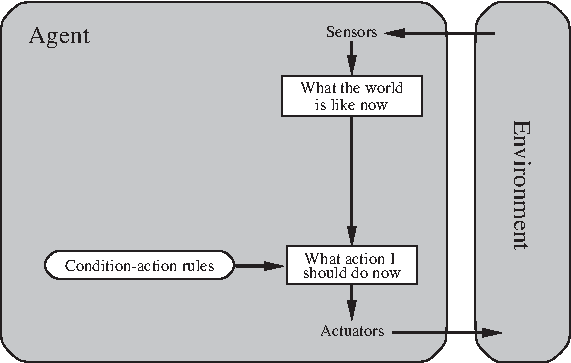
\includegraphics[width=0.5\textwidth]{img/agente-reativo-simples}
	\caption{Esquema geral de um agente reativo simples}
	\label{fig:agente-reativo-simples}
\end{figure}

O Algoritmo~\ref{alg:agente-reativo-simples} apresenta uma implementação básica para um agente reativo simples. A percepção é recebida através dos sensores do agente e é dada como entrada do algoritmo. A partir da percepção, é extraído o estado do ambiente (linha 2), que por sua vez serve de parâmetro para a seleção da regra correspondente (linha 3). Em geral, estes agentes selecionam a primeira regra cujas condições correspondem ao estado recuperado. A partir da regra selecionada, o agente extrai a ação a ser executada (linha 4), a qual é retornada e enviada aos atuadores.

\begin{algorithm}[h]
	\DontPrintSemicolon
	\Entrada{\textit{percepção}}
	\Saida{\textit{ação}}
	
	\Inicio{
		\textit{estado} $\gets$ INTERPRETAR-ENTRADA(\textit{percepção})\;
		\textit{regra} $\gets$ REGRA-CORRESPONDENTE(\textit{estado}, \textit{regras})\;
		\textit{ação} $\gets$ AÇÃO-DA-REGRA[\textit{regra}]\;
		\Retorna{\textit{ação}}
	}
	
	\caption{Pseudocódigo para um agente reativo simples}
	\label{alg:agente-reativo-simples}
\end{algorithm}

Podemos definir um agente reativo simples para o mundo do aspirador de pó. Dada sua simplicidade, o código deste agente pode ser ainda mais simples, uma vez que existem poucas regras. O Algoritmo~\ref{alg:agente-reativo-simples-aspirador} apresenta uma proposta de agente aspirador de pó reativo simples. Sempre que o estado da posição atual for \textit{Sujo}, o agente seleciona a ação \textit{Aspirar}. Caso contrário, ele move para o quadrado ao lado.

\begin{algorithm}[h]
	\DontPrintSemicolon
	\Entrada{\textit{percepção} na estrutura $[$\textit{posição},\,\textit{estado}$]$}
	\Saida{\textit{ação}}
	
	\Inicio{
		\Se{estado = Sujo}{
			\Retorna{\textit{Aspirar}}\;
		}\Senao{
			\Se{posição = A}{
				\Retorna{\textit{Direita}}\;
			}\Senao{
				\Retorna{\textit{Esquerda}}\;
			}
		}
	}
	
	\caption{Pseudocódigo para um agente aspirador de pó reativo simples}
	\label{alg:agente-reativo-simples-aspirador}
\end{algorithm}

Suponhamos que o sensor que determina a posição do robô estrague, levando-o a uma observação parcial do ambiente. Neste caso, o robô é capaz de apenas determinar se a posição em que se encontra está ou não com sujeira. Quando a posição estiver limpa, ele não consegue determinar para qual lado deve movimentar-se. Uma estratégia para superar esta dificuldade é fazer uso de \textbf{aleatoriedade} no momento de selecionar uma das ações de movimento. Ou seja, ele pode selecionar \textit{Direita} ou \textit{Esquerda} com probabilidade $0.5$. Em geral, agentes reativos simples possuem limitações, dada sua simplicidade, o que exige a adoção de técnicas como esta.


\subsection{Agentes reativos baseados em modelo}

Estes agentes são também chamados de \textbf{agentes deliberativos}. A ideia por trás dos agentes baseados em modelo consiste no agente ter uma representação do mundo (ambiente), de tal forma que ele entenda como o mundo funciona e como evolui com o passar do tempo. Um \textbf{modelo} é, portanto, a representação deste conhecimento que o agente possui do seu ambiente. Este modelo é construído e atualizado em função da sequência de percepções do agente. Neste sentido, o modelo é capaz de minimizar o problema da observação parcial do ambiente. Ou seja, caso o agente não consiga observar algum aspecto do ambiente, o modelo é capaz de determiná-lo (com certo nível de precisão).

A Figura~\ref{fig:agente-reativo-baseado-modelo} apresenta o esquema geral de um agente reativo baseado em modelo. Por ser um agente reativo, suas ações continuam sendo modeladas por regras condição-ação. No entanto, o agente mantém seu modelo do mundo (``como o mundo evolui'') que, juntamente com suas entradas sensoriais e as consequências de suas ações, serve para atualizar o estado percebido antes da tomada de decisão. Isto é, o estado é determinado pelas suas percepções do ambiente, seu conhecimento sobre aquilo que não foi possível perceber e as consequências da ação escolhida. Perceba que, para isso, o agente mantém uma representação interna do estado do ambiente.

\begin{figure}[h]
	\centering
	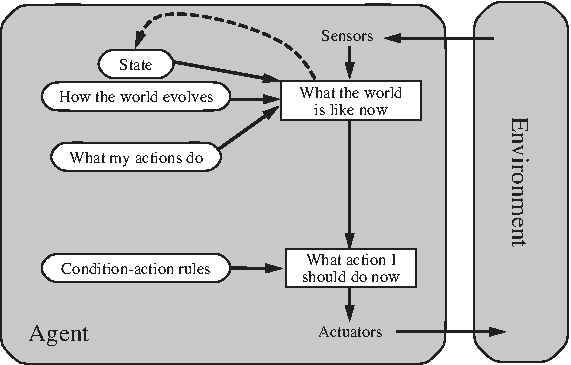
\includegraphics[width=0.5\textwidth]{img/agente-reativo-baseado-modelo}
	\caption{Esquema geral de um agente reativo baseado em modelo}
	\label{fig:agente-reativo-baseado-modelo}
\end{figure}

O Algoritmo~\ref{alg:agente-reativo-baseado-modelo} apresenta uma implementação básica para um agente reativo baseado em modelo. Em comparação com o pseudocódigo do agente reativo simples, a função \texttt{INTERPRETAR-ENTRADA} é substituída pela ação \texttt{ATUALIZAR-ESTADO} (linha 2). Antes, o agente só considerava suas percepções para definir o estado do ambiente. Agora, a percepção é utilizada em conjunto com o modelo e as ações do agente para determinar o estado do ambiente.

\begin{algorithm}[h]
	\DontPrintSemicolon
	\Entrada{\textit{percepção}}
	\Saida{\textit{ação}}
	
	\Inicio{
		\textit{estado} $\gets$ ATUALIZAR-ESTADO(\textit{estado}, \textit{ação}, \textit{percepção})\;
		\textit{regra} $\gets$ REGRA-CORRESPONDENTE(\textit{estado}, \textit{regras})\;
		\textit{ação} $\gets$ AÇÃO-DA-REGRA[\textit{regra}]\;
		\Retorna{\textit{ação}}
	}
	
	\caption{Pseudocódigo para um agente reativo baseado em modelo}
	\label{alg:agente-reativo-baseado-modelo}
\end{algorithm}

\subsection{Agentes baseados em objetivos}

Em muitos casos, não é suficiente manter uma representação do mundo e um conjunto de regras condição-ação. O agente pode deparar-se com situações de tomada de decisão em que é difícil definir a ação adequada. Neste caso, o agente deve manter um ou um conjunto de objetivos que descreva situações desejáveis. Por exemplo, um veículo autônomo que encontra um acidente de trânsito e precisa desviar seu caminho, escolhendo entre duas opções. Neste caso, seu objetivo é chegar no destino de sua viagem e a análise sobre qual rota tomar deve ser feita em função deste objetivo. Perceba que esta decisão não é tão simples como aquelas oriundas das regras condição-ação. Esta decisão deve considerar ações no futuro, definindo qual rota levará o agente a cumprir seu objetivo.

Os agentes baseados em objetivos são mais flexíveis, uma vez que o conhecimento que baliza suas decisões é representado explicitamente e pode ser facilmente modificado. Por exemplo, se começar a chover, o veículo autônomo tem o conhecimento de que o funcionamento do freio é alterado, bem como outros aspectos da dirigibilidade. Com isso, o veículo automaticamente ajusta todo o seu comportamento em função das novas condições climáticas. Para fazermos o mesmo com um agente reativo, teríamos que escrever um grande conjunto de regras condição-ação, que incluam a chuva como condição das novas ações.

\begin{figure}[h]
	\centering
	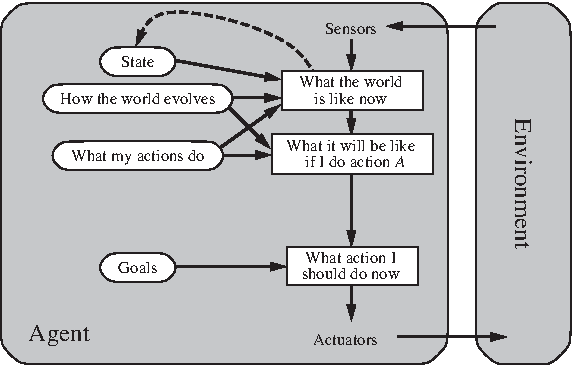
\includegraphics[width=0.5\textwidth]{img/agente-baseado-objetivos}
	\caption{Esquema geral de um agente baseado em objetivos}
	\label{fig:agente-baseado-objetivos}
\end{figure}

A Figura~\ref{fig:agente-baseado-objetivos} apresenta o esquema geral de um agente baseado em objetivos. Além de manter um estado interno, o modelo do seu ambiente e as consequências de suas ações, o agente mantém um conjunto de objetivos. Estes objetivos são utilizados na tomada de decisões, no lugar das regras condição-ação.

\subsection{Agentes baseados na utilidade}

Em geral, agentes baseados em objetivos utilizam seu conhecimento na tomada de decisões que atinjam seus objetivos. No entanto, esta abordagem não é suficiente para o desenvolvimento de agentes com alta qualidade. No exemplo do veículo autônomo, o agente escolherá pela rota que leve-o ao seu objetivo de chegar no destino da viagem. Se ambas as rotas o permitem chegar no seu destino, ele escolhe por qualquer uma das duas. Ou seja, seus objetivos servem para classificar as opções em alternativas de \textit{sucesso} e de \textit{insucesso}, na satisfação dos seus objetivos. Porém, se uma das rotas demora 5 minutos, enquanto a outra demora 30 minutos, é razoável optar pela primeira. Este comportamento não é obtido em um agente simples baseado em objetivos.

Para modelar este comportamento, definimos a \textbf{utilidade} como uma medida de recompensa na tomada de uma decisão. Neste sentido, a \textbf{função de utilidade} mapeia um estado (ou uma sequência de estados) em um número real que descreve o grau de sucesso (ou de felicidade) associado. Além de auxiliar na escolha de duas opções que levam ao objetivo, mas com graus de sucesso diferentes, a função de utilidade permite agir com inteligência em dois casos: (1) quando existem objetivos contraditórios e (2) quando incerteza no atingimento dos objetivos.
\begin{enumerate}[(1)]
	\item Considerando que o agente considera dois aspectos na escolha de rotas: tempo de viagem e desgaste do veículo. Se a primeira rota tem menor tempo e maior desgaste que a segunda, o agente terá que optar por um dos aspectos em detrimento do outro. A função de utilidade permite definir escolhas dessa natureza, onde o agente tem um compromisso com cada aspecto.
	\item Considerando que em ambas as rotas, não é certo que elas levam ao destino da viagem. Neste caso, a função de utilidade serve para definir a probabilidade de que cada rota leve ao destino, permitindo optar pela rota com maior valor de probabilidade.
\end{enumerate}

\begin{figure}[h]
	\centering
	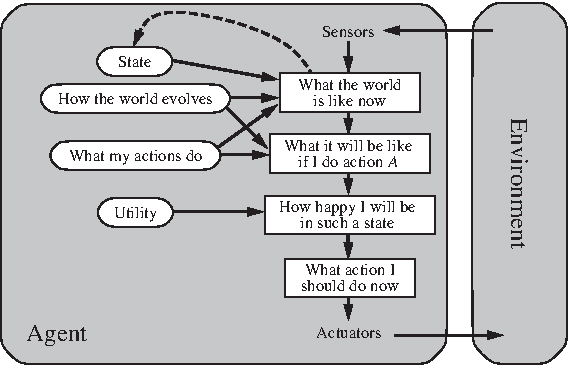
\includegraphics[width=0.5\textwidth]{img/agente-baseado-utilidade}
	\caption{Esquema geral de um agente baseado em utilidade}
	\label{fig:agente-baseado-utilidade}
\end{figure}

A Figura~\ref{fig:agente-baseado-utilidade} apresenta o esquema geral de um agente baseado em utilidade. Perceba que foram mantidos os componentes de um agente baseado em objetivos e que utiliza um modelo do mundo para tratar a observação parcial do ambiente. Agora, a tomada de decisão utiliza o conceito de utilidade para definir ``\textit{o quanto serei feliz em tal estado}'', optando pela ação que leva ao maior grau de felicidade. Em geral, agentes racionais utilizam esta estrutura interna, pois a racionalidade consiste em optar pela ação que maximiza os ganhos do agente, em termos de utilidade.

\subsection{Agentes com aprendizagem}

As seções anteriores apresentaram agentes com diferentes componentes, que definem a forma como eles se comportam. Em outras palavras, estes componentes definem a forma como as percepções são tratadas para a seleção de uma ação. Em agentes que aprendem com a experiência, são incluídos elementos que permitem ajustar os componentes citados, de tal forma que o comportamento seja aprimorado. A Figura~\ref{fig:agente-aprendizagem} mostra o esquema geral de um agente com aprendizagem, constituído por quatro componentes principais: \textit{elemento de desempenho}, \textit{elemento de aprendizado}, \textit{crítico} e \textit{gerador de problemas}.

\begin{figure}[h]
	\centering
	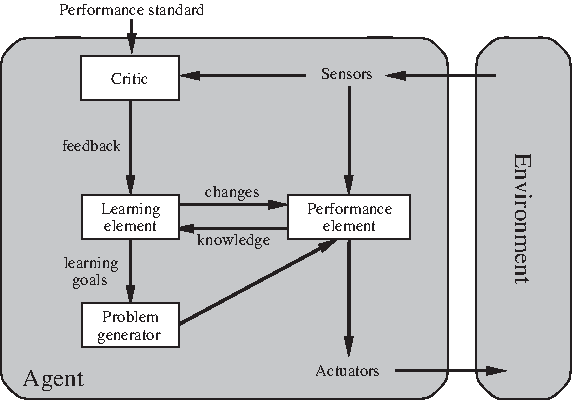
\includegraphics[width=0.5\textwidth]{img/agente-aprendizagem}
	\caption{Esquema geral de um agente com aprendizagem}
	\label{fig:agente-aprendizagem}
\end{figure}

O \textbf{elemento de desempenho} consiste na estrutura de tomada de decisão do agente, que recebe as percepções e delibera ações. Ou seja, este elemento contém uma das estruturas de componentes apresentadas nas seções anteriores (estrutura reativa simples, baseada em modelo, baseada em objetivos ou baseada na utilidade).

O \textbf{elemento de aprendizado} é responsável por ajustar o comportamento do agente, melhorando-o com o passar do tempo. Este elemento está em constante comunicação com o elemento de desempenho, pois sua tarefa é modificá-lo e receber o conhecimento obtido com a experiência. Por exemplo, o elemento de aprendizado cria novas regras e modifica as existentes no elemento de desempenho (considerando um agente reativo).

O \textbf{crítico} é responsável por medir o sucesso do agente sob o ponto de vista externo. Quando o agente executa uma determinada ação, o crítico informa o agente sobre o sucesso dela, de tal forma que o agente possa ajustar seu comportamento. Por exemplo, se o veículo autônomo fizer uma troca de pista brusca, ele atingiu seu objetivo interno de trocar de pista. No entanto, o ambiente externo (outros motoristas) mostra que não foi uma manobra segura. Esta consequência não é captada pelas percepções do agente e, portanto, é papel do crítico informar o elemento de aprendizado que esta manobra não deve ser realizada dessa forma. O elemento de aprendizado, por sua vez, inclui uma nova regra no elemento de desempenho, evitando situações similares no futuro. Ou seja, o agente aprendeu a não mudar de pista de forma brusca.

O \textbf{gerador de problemas} é responsável pelo comportamento exploratório do agente. Como vimos nas seções anteriores, o agente sempre seleciona a ação que lhe traz o maior retorno. Por exemplo, se uma rota leva ao destino e, no caso de uma segunda rota, não há certeza disso, o agente sempre seleciona a primeira rota. No entanto, se o agente explorar a segunda rota, pode descobrir um caminho mais curto para seu destino, ou descobrir que não é uma boa opção. Neste sentido, o gerador de problemas tem a tarefa de gerar situações de exploração, de tal forma que o agente aprenda com novas experiências.

\section{Recursos disponíveis}

Apesar de não ser necessário o uso de nenhuma tecnologia específica para o desenvolvimento de agentes, existem ferramentas que facilitam esta tarefa e fornecem uma arquitetura para a construção de agentes inteligentes. O Jason~\footnote{\url{http://jason.sourceforge.net/wp}} é uma extensão da linguagem AgentSpeak para o desenvolvimento de agentes e sistemas multiagentes. Outra linguagem bastante conhecida para o desenvolvimento de agentes em Java é o JADE~\footnote{\url{http://jade.tilab.com}}. O JaCaMo~\footnote{\url{http://jacamo.sourceforge.net}}, por sua vez, é um framework que combina a linguagem Jason com as tecnologias Cartago, para tratamento de artefatos, e Moise, para organizações de agentes.

Uma aplicação comum de sistemas multiagentes é a simulação de fenômenos do mundo real, área conhecida por simulação baseada em agentes. \cite{AbarEtAl2017} apresentam uma revisão atualizada dos softwares existentes para modelagem e simulação baseada em agentes. Uma ferramenta de destaque é o NetLogo~\footnote{\url{https://ccl.northwestern.edu/netlogo}}, que fornece um ambiente para o desenvolvimento de simulações baseadas em agentes de propósito geral. A linguagem fornece uma série de funções que facilitam o processo de desenvolvimento de sistemas dessa natureza.

\section{Exercícios}

\resetexercisenumbering

\begin{exercise}
Para cada uma das atividades (agente) abaixo, forneça uma descrição do ambiente de tarefa (medida de desempenho, ambiente, atuadores e sensores):
\begin{enumerate}[a.]
	\item Jogar futebol.
	\item Compra de livros usados de IA na Internet.
	\item Jogar uma partida de tênis.
	\item Praticar tênis contra uma parede.
	\item Realizar um salto em altura.
	\item Licitações de um item em um leilão.
\end{enumerate}
\end{exercise}

\begin{exercise}
Classifique os ambientes a seguir em: completamente observável ou parcialmente observável, determinístico ou estocástico (ou ainda, estratégico), episódico ou sequencial, estático ou dinâmico (ou ainda, semi-dinâmico), discreto ou contínuo, monoagente ou multiagente.

\begin{enumerate}[a.]
	\item Jogo de palavras cruzadas.
	\item Xadrez com relógio.
	\item Pôquer.
	\item Gamão.
	\item Veículo autônomo.
	\item Diagnóstico médico.
	\item Análise de imagens.
	\item Robô de seleção de peças.
	\item Controlador de refinaria.
	\item Instrutor interativo de inglês.
\end{enumerate}
\end{exercise}

\begin{exercise}
Implemente um simulador para o ambiente do aspirador de pó. Sua implementação deve ser modular, de forma que os sensores, atuadores e as características do ambiente (tamanho, forma, localização da sujeira, etc.) possam ser alterados facilmente.
\end{exercise}

\begin{exercise}
Implemente um agente reativo simples para o ambiente do aspirador de pó, usando o simulador desenvolvido no exercício anterior. Execute as simulações com diferentes posições de sujeira e de início do agente. Registre a pontuação de desempenho do agente para cada configuração e sua pontuação média global.
\end{exercise}

\begin{exercise}
Considere uma versão modificada do ambiente de aspirador de pó, na qual o agente é penalizado com um ponto para cada movimento.
\begin{enumerate}[a.]
	\item Um agente reativo simples pode ser perfeitamente racional para esse ambiente? Explique.
	\item E um agente reativo com estado? Projete tal agente.
	\item Como suas respostas para os itens \textbf{a} e \textbf{b} mudarão se as percepções do agente fornecerem o status limpo/sujo de cada quadrado do ambiente?
\end{enumerate}
\end{exercise}

\begin{exercise}
Considere uma versão modificada do ambiente de aspirador de pó, na qual a geografia do ambiente (extensão, limites e obstáculos) é desconhecida, bem como a configuração inicial de sujeira. Neste caso, o agente não se movimenta apenas para os lados, mas também para baixo e para cima.
\begin{enumerate}[a.]
	\item Um agente reativo simples pode ser perfeitamente racional para esse ambiente? Explique.
	\item Um agente reativo simples com uma função de agente \textit{aleatório} pode superar um agente reativo simples? Implemente tal agente e faça a medição de seu desempenho em vários ambientes.
	\item Você poderia projetar um ambiente no qual seu agente aleatório terá um desempenho muito ruim? Mostre seus resultados.
	\item Um agente reativo com estados pode superar um agente reativo simples? Implemente tal agente e faça a medição de seu desempenho em vários ambientes.
\end{enumerate}

\end{exercise}